\chapter{Benutzeroberfläche}
\setcounter{counterKriterien}{0}


\gls{OQAT} stellt dem Nutzer eine intuitive graphische Oberfläche zur Verfügung.

\begin{figure}[p]
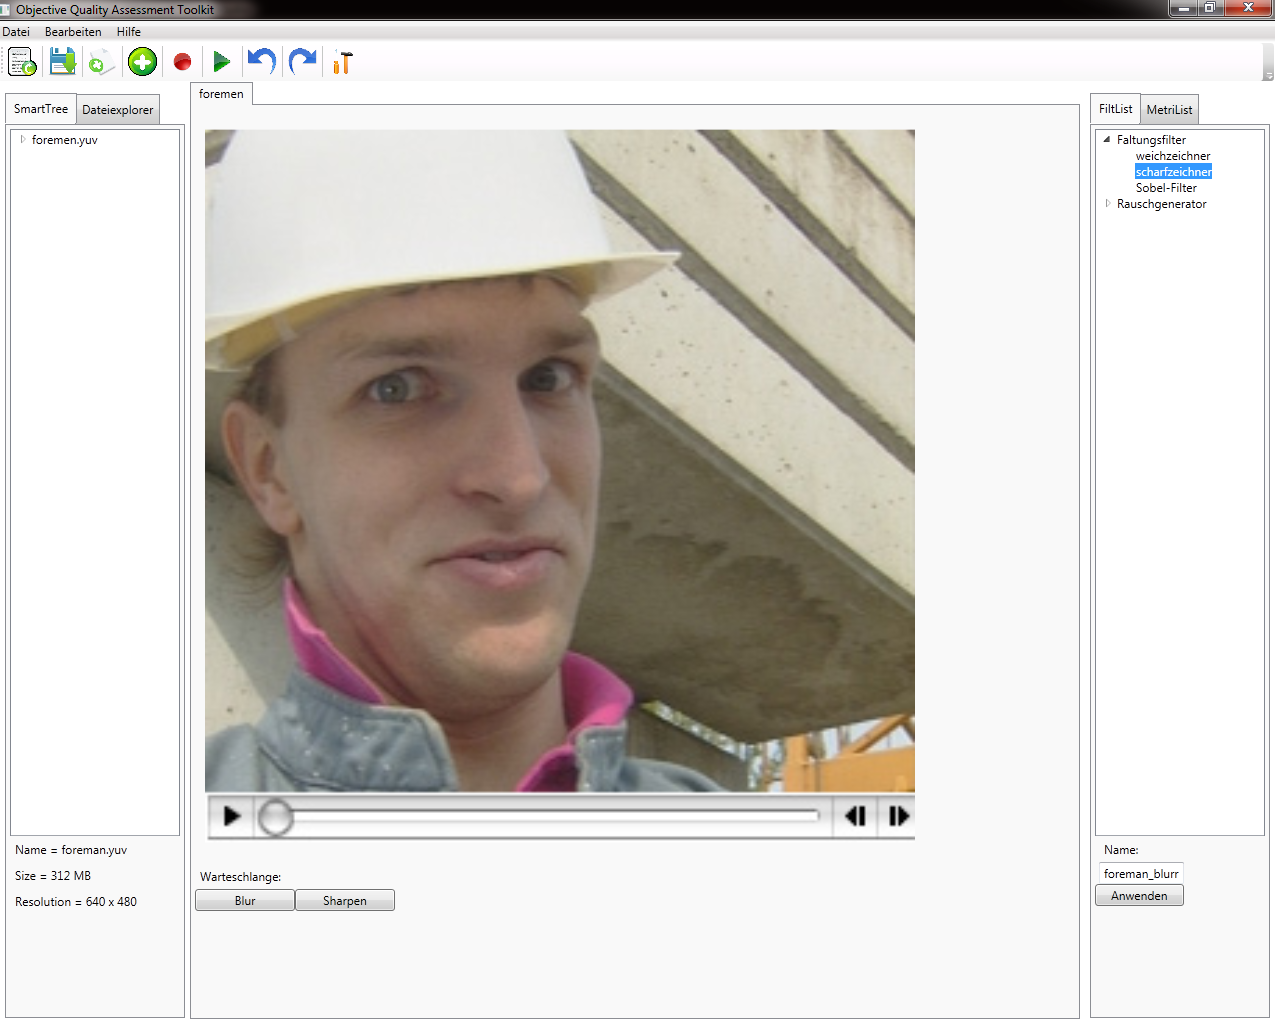
\includegraphics[scale=0.35]{bilder/screenFilter.png}
\caption{Auswahl mehrerer Filter und des Namens unter dem das so entstandene Video im
Projektordner gespeichert werden soll}
\label{screenFilter}
\end{figure}
\begin{figure}[p]
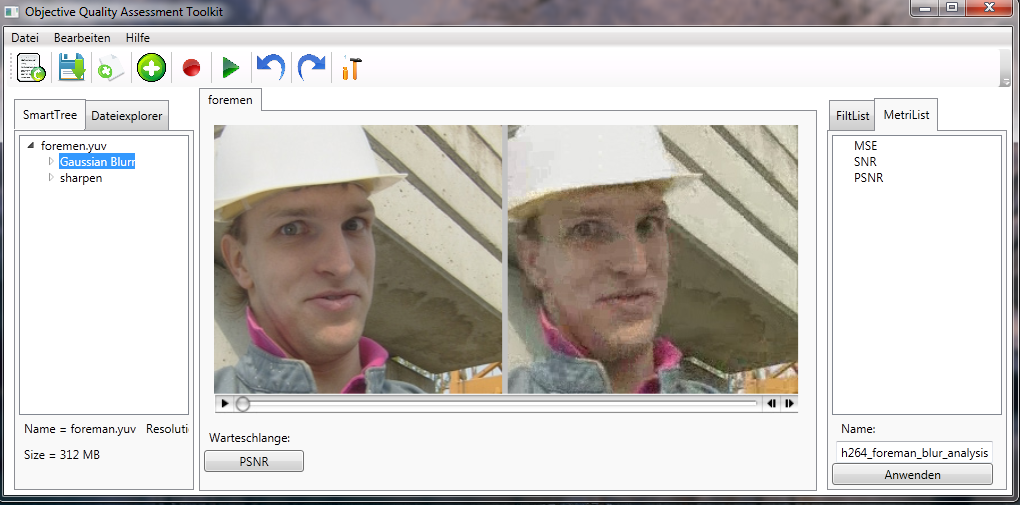
\includegraphics[scale=0.6]{bilder/screenAnalys.png}
\caption{Auswahl einer Analysemetrik und des Namens unter dem die Ergebnisdaten im 
Projektordner abgelegt werden sollen}
\label{screenAnalys}
\end{figure}
\begin{figure}[p]
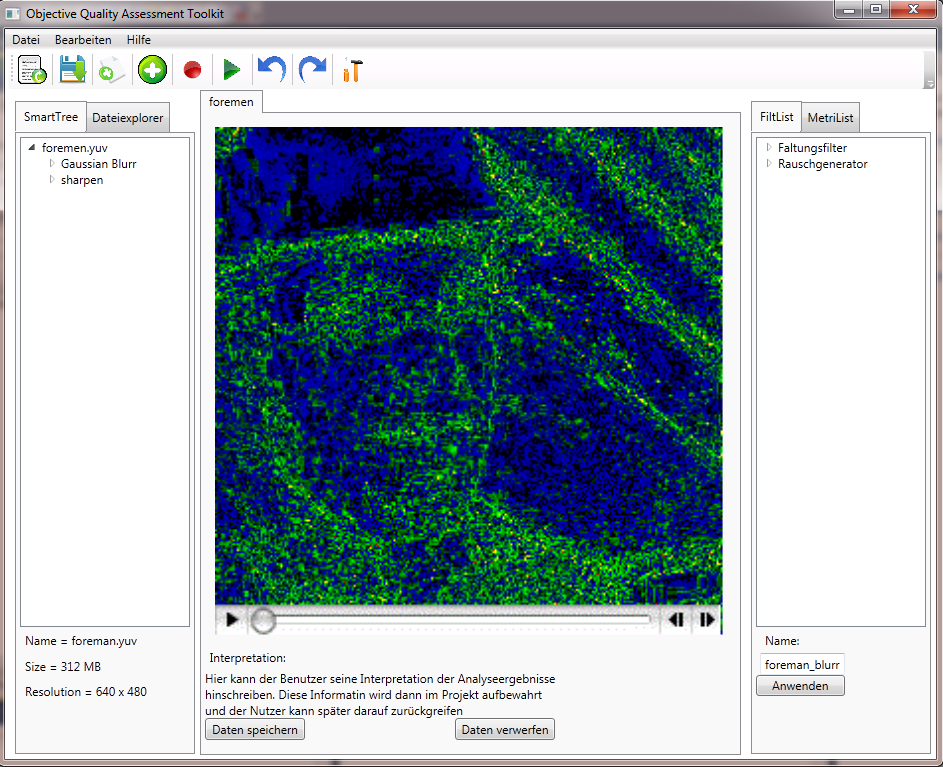
\includegraphics[scale=0.6]{bilder/screenResults.png}
\caption{Visuelle Darstellung der Ergebnisse nach einem Analysevorgang mit der \gls{psnr} Metrik}
\label{screenResults}
\end{figure}
